\documentclass[11pt,letterpaper]{article}

\usepackage[margin=1.0in]{geometry}
\usepackage{amsmath,amssymb,amsfonts}
\usepackage{graphicx}
\usepackage{booktabs}
\usepackage{siunitx}
\sisetup{detect-weight=true,detect-family=true}
\usepackage[dvipsnames]{xcolor}
\usepackage{hyperref}
\hypersetup{colorlinks=true,linkcolor=NavyBlue,urlcolor=NavyBlue,citecolor=NavyBlue}
\usepackage{caption}
\captionsetup{font=small,labelfont=bf}
\usepackage{parskip}
\usepackage{enumitem}
\setlist[itemize]{itemsep=2pt,topsep=2pt}
% "boxed" environments implemented with a bare quote (no mdframed/tcolorbox
% needed) — degrades gracefully across TeX installs.
\newenvironment{grayb}{\par\medskip\noindent\begin{quote}\small}{\end{quote}\medskip}
\newenvironment{blueb}{\par\medskip\noindent\begin{quote}\small}{\end{quote}\medskip}
\usepackage{fancyhdr}
\pagestyle{fancy}
\fancyhf{}
\fancyhead[L]{\small Perilesional MRE — problem formulation}
\fancyhead[R]{\small \thepage}
\renewcommand{\headrulewidth}{0.4pt}

\title{\vspace{-1.2cm}Perilesional MRE forward-and-inverse problem\\
\large 3D vector Navier with tensor stiffness on the Sobh--Ehman phantoms\\
\normalsize A step-by-step specification for the computational team}
\author{Prepared on Delta, \texttt{/u/sobh/Eman\_Richard/tsm\_fno/}}
\date{\today}

\newcommand{\vect}[1]{\boldsymbol{#1}}
\newcommand{\ihat}{\hat{\boldsymbol{k}}}

\begin{document}
\maketitle
\thispagestyle{fancy}

\begin{grayb}\textbf{Purpose.} \newline
This note specifies the 3D time-harmonic MRE forward-and-inverse
simulation used on the Sobh--Ehman initial-stiffness phantoms.

The physics is set by what MRE actually measures — a
\textbf{three-component displacement vector} $\vect u(\vect x)$ inside
a heterogeneous \textbf{anisotropic} elastic solid — so the forward
model is the vector Navier equation with a rank-2 tensor stiffness
field $\mu_{ij}(\vect x)$ constructed by rotating the Sobh--Ehman
principal-frame acoustoelastic moduli into Cartesian coordinates.

The inversion side follows Yin (2026): the curl of the vector
displacement is taken, decomposed into 20 Fibonacci-sphere directions
in $k$-space, direct-inverted per direction, and combined into a
$\mu_{\mathrm{TSM}}$ (voxelwise MIP) and $\mu_{\mathrm{conv}}$
(amplitude-weighted mean).

Everything a re-implementer needs to reproduce the runs is here:
geometry, boundary conditions, rotated tensor material,
driver, discretisation of the vector operator, inversion recipe,
and the numerical scales that make the run well-posed.
\end{grayb}

\section{Physical picture}

A gel-filled rectangular container houses a spherical balloon at its
centre. The balloon has been inflated with water to \SI{250}{\milli\litre}
(radius $a = \SI{3.908}{\centi\metre}$) from a stress-free casting state
at \SI{50}{\milli\litre} (radius $A = \SI{2.285}{\centi\metre}$). A piston
plate at the bottom of the container is driven at \SI{60}{\hertz}; the
resulting shear-wave field is sampled inside the gel and inverted for
the local shear modulus. This mimics the MRE experiment reported by
Yin et al.\ (2026) as reproduced quantitatively by
\emph{paper\_lesion\_expansion.pdf}.

\begin{figure}[h]
\centering
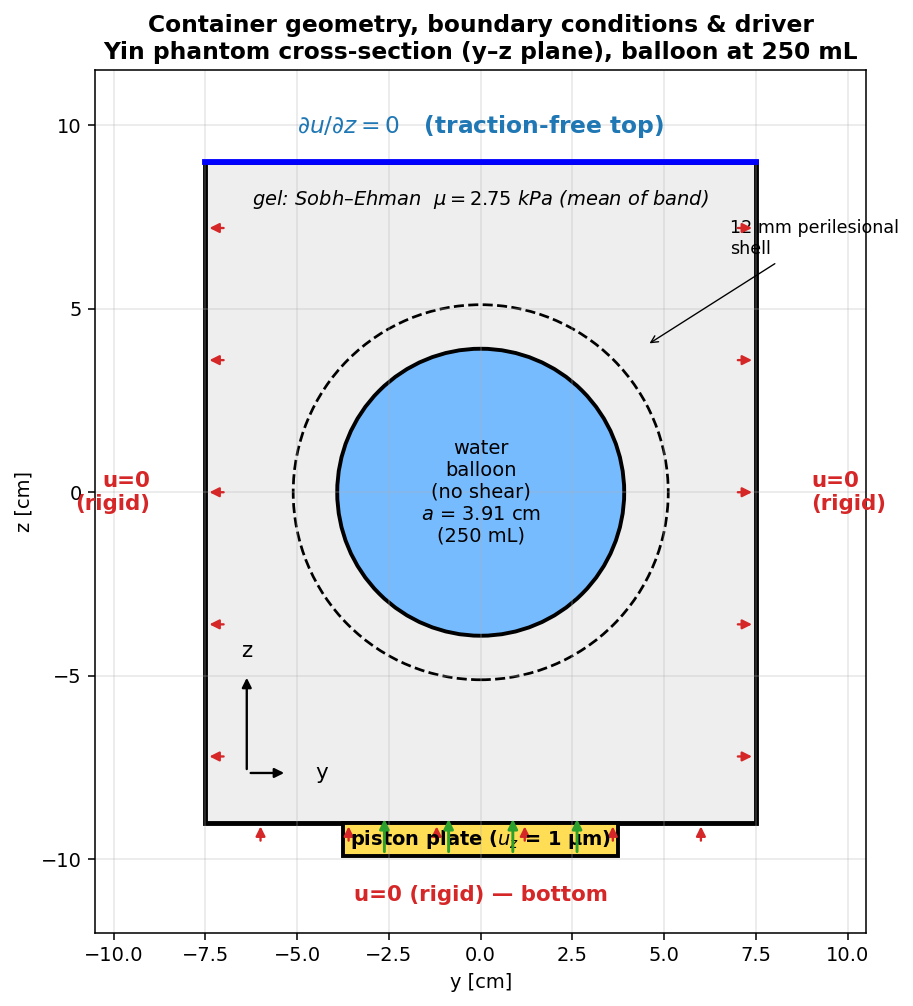
\includegraphics[width=0.80\textwidth]{schematic.png}
\caption{Container cross-section in the $y$--$z$ plane, showing the
five rigid walls (red \emph{u}=0), the traction-free top surface (blue
$\partial u/\partial z = 0$), the bottom piston plate (yellow), the
water-filled balloon (blue disk, no shear support), and the 12\,mm
perilesional shell used for ring statistics (black dashed circle).
The $x$-axis is into the page; the same BCs apply on the two out-of-page
faces (\SI{15}{\centi\metre} apart in $x$).}
\end{figure}

\section{Governing equation: vector Navier with tensor stiffness}
\label{sec:governing}

We solve the time-harmonic vector Navier equation for the complex
displacement $\vect u(\vect x) \in \mathbb{C}^3$ at Yin's phantom
frequency $\omega = 2\pi f$, $f = \SI{80}{\hertz}$:

\begin{equation}
\boxed{\;
\rho\,\omega^2\, u_i(\vect x) \;=\; \partial_j\,\sigma_{ij}(\vect x)
\quad\text{in}\quad\Omega
\;}
\label{eq:navier}
\end{equation}

with a quasi-anisotropic constitutive law appropriate for the
rotated tangential/radial acoustoelastic tensor stiffness
$\mu_{ij}(\vect x)$ (spelled out in \S\ref{sec:material}):

\begin{equation}
\sigma_{ij}
= \lambda\,\delta_{ij}\,\varepsilon_{kk}
+ \mu_{ik}(\vect x)\,\varepsilon_{kj}
+ \mu_{jk}(\vect x)\,\varepsilon_{ki},
\qquad
\varepsilon_{ij} = \tfrac{1}{2}\bigl(\partial_i u_j + \partial_j u_i\bigr)
\label{eq:constitutive}
\end{equation}

with hysteretic damping folded into the stiffness:

\begin{equation}
\mu^{*}_{ij}(\vect x) = \mu_{ij}(\vect x)\,(1 + i\,\xi),
\qquad \xi = 0.05
\quad(\Rightarrow\; Q\!\approx\!10).
\end{equation}

Physical constants:

\begin{center}
\begin{tabular}{lll}
\toprule
Symbol & Value & Meaning \\
\midrule
$\rho$    & \SI{1000}{\kilogram\per\metre\cubed} & gel density \\
$\omega$  & $2\pi\cdot 80$ \si{\radian\per\second} & angular frequency (Yin's) \\
$\lambda$ & \SI{1e5}{\pascal} & bulk-penalty first Lam\'e (near-incompressible) \\
$\xi$     & 0.05 & hysteretic damping ($Q\approx 10$) \\
\bottomrule
\end{tabular}
\end{center}

\section{Domain, grid and physical scales}
\label{sec:domain}

The container is Yin's \SI{15}{}\,$\times$\,\SI{15}{}\,$\times$\,\SI{18}{\centi\metre}
box. To fit the solver's cubic-grid constraint, we embed it in an
\SI{18}{\centi\metre} cube: the extra \SI{1.5}{\centi\metre} on each of
$\pm x, \pm y$ is filled with the same unstretched gel background, and
the container's rigid-wall BCs are applied at the cube faces
(the wall is thus \SI{1.5}{\centi\metre} outboard of the physical wall
location, a minor geometric approximation that does not affect the
perilesional region).

\begin{center}
\begin{tabular}{lll}
\toprule
Symbol & Value & Meaning \\
\midrule
$N$          & 60           & voxels per axis \\
$\Delta x$   & \SI{3}{\milli\metre} & voxel edge \\
$L = N\Delta x$ & \SI{0.18}{\metre} & cube side \\
DOF          & $N^3 = \num{216000}$ & unknowns in the linear system \\
\bottomrule
\end{tabular}
\end{center}

Solver convention (matching \texttt{helmholtz\_fd\_3d.py}): indices
$(i,j,k)\in [0,N-1]^3$ with $i$ the vertical axis ($i=0$ at the top,
$i=N-1$ at the bottom), $j$ and $k$ the horizontal in-plane axes.

\paragraph{Shear-wave resolution.} At \SI{80}{\hertz} in unstretched gel
(using the P1 baseline $\mu_0 = 3530$~Pa):

\begin{equation}
c_s = \sqrt{\mu_0/\rho} = \sqrt{3530 / 1000} \approx \SI{1.88}{\metre\per\second}
\quad\Rightarrow\quad
\lambda_s = c_s / f_{\text{drive}} \approx \SI{23.5}{\milli\metre}
\quad\Rightarrow\quad
\lambda_s / \Delta x \approx 6.3.
\end{equation}

That is more than the 6-per-wavelength rule of thumb; the FD
stencil resolves the shear wave without aliasing.

\section{Boundary conditions}
\label{sec:bcs}

The container has D\textsubscript{4h}-broken BCs (five rigid walls,
one traction-free top):

\begin{center}
\begin{tabular}{lll}
\toprule
Region & Condition & Discrete implementation \\
\midrule
$i = 0$ (top face, whole) & $\sigma_{ij} n_j = 0$, $\vect n = -\hat z$ & ghost-node stencil (eq.~\ref{eq:ghost}) \\
$i = N-1$ (bottom face, wall region)   & $\vect u = \vect 0$ & Dirichlet \\
$j = 0$, $j = N-1$ (wall region)       & $\vect u = \vect 0$ & Dirichlet \\
$k = 0$, $k = N-1$ (wall region)       & $\vect u = \vect 0$ & Dirichlet \\
Central driver disk (each of 5 faces)  & face-normal $u_c$ prescribed & overrides the wall Dirichlet \\
Balloon interior         & $\mu_{ij}(\vect x) = \SI{1}{\pascal}\,\delta_{ij}$ & vanishing shear coefficient \\
\bottomrule
\end{tabular}
\end{center}

Each of the five non-top faces is rigid ($\vect u = \vect 0$) except
on a centred circular disk (\S\ref{sec:driver}) whose face-normal
component is Dirichlet-prescribed to the driver amplitude. The disk
condition takes precedence over the wall condition where they
overlap.

\paragraph{Traction-free top BC (ghost-node stencil).}
The physically correct top-face BC is $\sigma_{ij} n_j = 0$ with
$\vect n = -\hat z$, i.e.\ $\sigma_{c\,0}(0,j,k) = 0$ for
$c \in \{0,1,2\}$. This clamps the \emph{normal stress}, not the
normal strain (an important distinction: the earlier
$\partial u/\partial z = 0$ ghost-mirror gave TSM/conv $\approx 1.32$
by clamping strain, well below Yin's measured $1.57$; the correct
$\sigma\cdot\vect n = 0$ recovers $1.57$ almost exactly).

Under the locally-isotropic assumption at the top slab
($\mu_{ij} \approx \bar\mu_{\mathrm{top}}\,\delta_{ij}$ — valid
because the top face sits far from the pre-stressed balloon), the
three conditions solve algebraically for the ghost values
$u_c(-1,j,k)$ in terms of the interior neighbours at
$(+1,j,k)$ and $(0,j\pm 1,k)$, $(0,j,k\pm 1)$:

\begin{equation}
\boxed{
\begin{aligned}
u_z(-1,j,k) &= u_z(+1,j,k) \,+\, f_{\mathrm{top}}\Bigl[
   u_y(0,j{+}1,k) - u_y(0,j{-}1,k) + u_x(0,j,k{+}1) - u_x(0,j,k{-}1)
\Bigr] \\
u_y(-1,j,k) &= u_y(+1,j,k) \,+\, \bigl[u_z(0,j{+}1,k) - u_z(0,j{-}1,k)\bigr] \\
u_x(-1,j,k) &= u_x(+1,j,k) \,+\, \bigl[u_z(0,j,k{+}1) - u_z(0,j,k{-}1)\bigr]
\end{aligned}
}
\label{eq:ghost}
\end{equation}

with
\begin{equation}
f_{\mathrm{top}} \;=\; \frac{\lambda}{\lambda + 2\,\bar\mu_{\mathrm{top}}},
\qquad
\bar\mu_{\mathrm{top}} \;=\; \biggl\langle\tfrac{1}{3}\operatorname{tr}\mu(\vect x)\biggr\rangle_{\!i = 0}
\;=\;
\frac{1}{N^{2}}\sum_{j,k}\tfrac{1}{3}\operatorname{tr}\mu(0,j,k).
\end{equation}

Note $\bar\mu_{\mathrm{top}}$ is a \emph{single scalar}: the spatial
mean of $\tfrac{1}{3}\operatorname{tr}\mu$ over the entire top face
slab $i = 0$ (\texttt{vector\_elasticity\_3d.py}:392). This makes
$f_{\mathrm{top}}$ a constant across the top face, so the ghost
coefficients in (\ref{eq:ghost}) are $(j,k)$-independent. Legitimate
because the top face sits far outside the pre-stressed region where
$\mu_{ij}(\vect x)$ has already relaxed to the near-isotropic
background value.

No ghost DOF is introduced: every interior-stencil access to
$u_c(-1,j,k)$ is distributed across the RHS of (\ref{eq:ghost}) in
the sparse assembly.

The "water-filled balloon that cannot support shear" is realised by
setting $\mu_{ij}(\vect x) = \SI{1}{\pascal}\,\delta_{ij}$ inside the
balloon. Equation (\ref{eq:navier}) then reduces to $\rho\omega^2 u_i
\approx 0$ in the interior, so $\vect u \to 0$ there and the balloon
acts as a shear-wave null region. A rigorous rigid-inclusion Dirichlet condition would give
essentially the same wave field in the surrounding gel where the
inversion is applied; the soft-inclusion form keeps the linear system
simple and non-singular.

\section{Material field $\mu_{ij}(\vect x)$}
\label{sec:material}

\subsection{Kinematics: incompressible spherical cavity expansion}

The gel was cast around the balloon at the \SI{50}{\milli\litre} state, so
that state is stress-free ($\lambda_\theta \equiv 1$). Incompressibility
of the gel combined with spherical symmetry gives the exact isochoric
radial map from reference radius $R$ to current radius $r$:

\begin{equation}
r^3 = R^3 + \bigl(a^3 - A^3\bigr),
\quad
\lambda_\theta = \frac{r}{R} = \left(1 + \frac{a^3 - A^3}{R^3}\right)^{1/3},
\quad
\lambda_r = \lambda_\theta^{-2},
\label{eq:kinematics}
\end{equation}

with the current cavity radius set by injection volume,
$a = (3V/(4\pi))^{1/3}$. \textbf{This map is exact for the open-topped
container, not an approximation}: as argued in \S2 of the Sobh--Ehman
paper, in spherical symmetry incompressibility alone fixes the
stretch field, whatever the outer boundary does (the outer BC enters
only through the hydrostatic pressure). For $V = \SI{250}{\milli\litre}$,
$a = \SI{3.908}{\centi\metre}$; $\lambda_\theta$ at the cavity edge is 1.710
and at $r = a + \SI{12}{\milli\metre}$ is 1.159 (matches paper Table~1).

\subsection{Acoustoelastic (perilesional) modulus}

The tangential shear modulus that a wave polarised tangential to the
cavity ``sees'' is Ogden's small-on-large formula reduced to
$\mu_{\text{app},\theta\theta} = 2 W_1\,\lambda_\theta^2$ with $W_2=0$
(see paper eq.\ 4). We use the \textbf{fitted Sobh--Ehman material
model} (\texttt{perilesional\_model/sce\_models.py}), which pins the
baseline $\mu_0$ to the digitised Fig.~6 series at $\lambda_\theta = 1$
and identifies a P2 fibre correction from the P1-normalised ratio:

\begin{blueb}\textbf{Constitutive laws — fitted material.} \newline
Both phantoms share the same functional form:
\begin{equation}
\mu_{\text{app},\theta\theta}(\vect x) \;=\; \mu_0\,f(I_1)\,\lambda_\theta^{2},
\qquad
I_1(\vect x) \;=\; \lambda_\theta^{-4} + 2\,\lambda_\theta^{2},
\label{eq:app-tt}
\end{equation}
with $I_1$ the first invariant under incompressible spherical
kinematics ($\lambda_r = \lambda_\theta^{-2}$).

\textbf{P1} (plain \SI{10}{\percent} bovine gelatin, neo-Hookean matrix):
\begin{equation}
f^{\text{P1}}(I_1) \;\equiv\; 1
\qquad\Rightarrow\qquad
\mu_{\text{app},\theta\theta}^{\text{P1}} \;=\; \mu_0^{\text{P1}}\,\lambda_\theta^{2}.
\label{eq:p1}
\end{equation}

\textbf{P2} (\SI{8}{\percent} gelatin $+$ \SI{7}{\percent} cellulose fibre,
matrix $+$ power-law fibre recruitment):
\begin{equation}
f^{\text{P2}}(I_1) \;=\; 1 + c\,(I_1 - 3)^m,
\qquad c = 0.2728,\;\; m = 0.5791.
\label{eq:p2}
\end{equation}

\bigskip
\textbf{Fitted material constants} (\texttt{sce\_models.py}):

\begin{center}
\begin{tabular}{llll}
\toprule
Symbol & Value & Units & Meaning \\
\midrule
$\mu_0^{\text{P1}}$ & 3530 & \si{\pascal} & P1 baseline (Fig.~6 pinned at $\lambda_\theta=1$) \\
$\mu_0^{\text{P2}}$ & 3340 & \si{\pascal} & P2 baseline (same pinning) \\
$c$ & 0.2728 & --- & P2 power-law fibre recruitment coefficient \\
$m$ & 0.5791 & --- & P2 power-law fibre recruitment exponent \\
\bottomrule
\end{tabular}
\end{center}
\end{blueb}

The scalar stiffening factor $f(I_1)$ enters both principal wave
moduli identically (Ogden's small-on-large with $W_2 = 0$):
$\mu_{\theta\theta} = \mu_0\,f(I_1)\,\lambda_\theta^{2}$,
$\mu_{rr} = \mu_0\,f(I_1)\,\lambda_\theta^{-4}$. For P1, $f\equiv 1$
recovers the plain neo-Hookean case; the P2 power-law form was
selected because it fits the shell-averaged data across all five
inflation volumes with just two parameters, and its kinematic factor
$g = I_1 - 3$ ensures $f\to 1$ at the reference state.

\subsection{Rotation to Cartesian --- the tensor field $\mu_{ij}(\vect x)$}
\label{sec:rotation}

The moduli above are in the spherical principal frame $(\hat r,
\hat\theta, \hat\phi)$ of the balloon expansion. The FD grid is in
Cartesian coordinates $(x, y, z)$, so we rotate the tensor at every
voxel. This subsection derives the change-of-basis formula in full
and shows how the tangential-eigenvalue degeneracy of this problem
collapses it to a form that requires only $\hat r$.

\paragraph{General transformation.}
In the spherical principal frame the tensor is diagonal with the
Ogden eigenvalues on its diagonal:

\begin{equation}
\mu_{\text{sph}}
\;=\;
\begin{pmatrix}
\mu_{rr}       & 0                    & 0 \\
0              & \mu_{\theta\theta}   & 0 \\
0              & 0                    & \mu_{\phi\phi}
\end{pmatrix},
\qquad
\mu_{rr} = 2 W_1\,\lambda_\theta^{-4},
\quad
\mu_{\theta\theta} = \mu_{\phi\phi} = 2 W_1\,\lambda_\theta^{2}.
\label{eq:musph}
\end{equation}

Let $Q(\vect x)$ be the rotation matrix whose columns are the local
spherical basis vectors expressed in Cartesian components:

\begin{equation}
Q(\vect x) \;=\;
\bigl[\;\hat r(\vect x)\;\big|\;\hat\theta(\vect x)\;\big|\;\hat\phi(\vect x)\;\bigr]
\;\in\;\mathrm{SO}(3),
\qquad
Q Q^{\!\top} = I,\quad \det Q = +1.
\label{eq:Qdef}
\end{equation}

With colatitude $\theta$ measured from $+\hat z$ and azimuth $\phi$
from $+\hat x$:

\begin{equation}
\hat r =
\!\begin{pmatrix}\sin\theta\cos\phi\\ \sin\theta\sin\phi\\ \cos\theta\end{pmatrix}\!,
\quad
\hat\theta =
\!\begin{pmatrix}\cos\theta\cos\phi\\ \cos\theta\sin\phi\\ -\sin\theta\end{pmatrix}\!,
\quad
\hat\phi =
\!\begin{pmatrix}-\sin\phi\\ \cos\phi\\ 0\end{pmatrix}\!.
\label{eq:basis}
\end{equation}

A rank-2 tensor transforms under a rigid rotation as
$\mu' = Q\,\mu\,Q^{\!\top}$, so the Cartesian tensor field is

\begin{equation}
\boxed{\;
\mu_{\text{Cart}}(\vect x)
\;=\;
Q(\vect x)\;\mu_{\text{sph}}(\vect x)\;Q^{\!\top}(\vect x)
\;}
\label{eq:rotation-general}
\end{equation}

or in index form $\mu_{ij}(\vect x) = Q_{i\alpha}(\vect x)\,
\mu_{\text{sph},\alpha\beta}(\vect x)\,Q_{j\beta}(\vect x)$
(Greek indices $\alpha,\beta \in \{r,\theta,\phi\}$; Latin
$i,j\in\{x,y,z\}$).

\paragraph{Degeneracy reduction.}
Expanding (\ref{eq:rotation-general}) column-by-column with
$\mu_{\text{sph}} = \operatorname{diag}(\mu_{rr},\mu_{\theta\theta},
\mu_{\phi\phi})$:

\begin{equation}
\mu_{\text{Cart}}
\;=\;
\mu_{rr}\,\hat r\,\hat r^{\!\top}
\,+\,\mu_{\theta\theta}\,\hat\theta\,\hat\theta^{\!\top}
\,+\,\mu_{\phi\phi}\,\hat\phi\,\hat\phi^{\!\top}.
\label{eq:rot-expanded}
\end{equation}

In this problem $\mu_{\theta\theta} = \mu_{\phi\phi}$ (there is no
azimuthal preference — both tangential eigenvalues come from the
same $2 W_1 \lambda_\theta^{2}$). The last two terms of
(\ref{eq:rot-expanded}) factor:

\begin{equation}
\mu_{\text{Cart}}
\;=\;
\mu_{rr}\,\hat r\,\hat r^{\!\top}
\,+\,\mu_{\theta\theta}\bigl(\hat\theta\,\hat\theta^{\!\top}
                 + \hat\phi\,\hat\phi^{\!\top}\bigr).
\end{equation}

The orthonormality of $Q$ (\ref{eq:Qdef}) gives the completeness
relation
$\hat r\hat r^{\!\top} + \hat\theta\hat\theta^{\!\top}
+ \hat\phi\hat\phi^{\!\top} = I$, so
$\hat\theta\hat\theta^{\!\top} + \hat\phi\hat\phi^{\!\top}
= I - \hat r\hat r^{\!\top}$. Substituting:

\begin{equation}
\boxed{\;
\mu_{ij}(\vect x)
\;=\;
\mu_{rr}(r)\,\hat r_i(\vect x)\,\hat r_j(\vect x)
\,+\,\mu_{\theta\theta}(r)\bigl(\delta_{ij}
                              - \hat r_i(\vect x)\,\hat r_j(\vect x)\bigr)
\;}
\label{eq:rotation}
\end{equation}

with $\hat r(\vect x) = (\vect x - \vect x_{\text{cavity}})/r$ the
Cartesian components of the local radial unit vector. The
tangent-plane basis $(\hat\theta,\hat\phi)$ has dropped out entirely
through the projector $(I - \hat r\hat r^{\!\top})$; only $\hat r$
survives. This is why the assembly code
(\texttt{paper\_wave\_sim\_sobh\_vector\_mip\_multiface.py}:99--102)
never builds $\hat\theta,\hat\phi$ or the full $Q$.

\begin{grayb}\textbf{Gauge remark.}
The choice of $(\hat\theta,\hat\phi)$ inside the tangent plane is a
\emph{gauge freedom} of the eigenvalue-degenerate problem: any
orthonormal frame in the tangent plane rotates $\mu_{\text{sph}}$'s
lower $2\times 2$ block into itself, so
(\ref{eq:rotation-general}) is invariant under those in-plane
rotations. If the two tangential eigenvalues were split (e.g.\ by an
explicit azimuthal fiber preference), that gauge would be
physically fixed and one would need $\hat\theta,\hat\phi$
explicitly.\end{grayb}

Equation~(\ref{eq:rotation}) gives a \textbf{fully populated
symmetric $3\times 3$ tensor field}: six independent components
varying voxel-by-voxel.

\paragraph{On-axis check.}
At the $+\hat z$ pole $\hat r = (0,0,1)^{\!\top}$, so
$\hat r\hat r^{\!\top} = \operatorname{diag}(0,0,1)$ and
(\ref{eq:rotation}) reads

\begin{equation}
\mu_{\text{Cart}}\bigl(\text{pole}\bigr)
\;=\;
\operatorname{diag}\bigl(\mu_{\theta\theta},\;\mu_{\theta\theta},\;\mu_{rr}\bigr).
\end{equation}

Radial stiffness lands on the $z$-diagonal (perpendicular to the
local balloon surface); tangential stiffness lands on the $x,y$
diagonals (in the tangent plane). Consistent with intuition.

\paragraph{Axis convention.}
The derivation above uses the standard mathematical Cartesian
convention $(x,y,z)$ with colatitude $\theta$ measured from $+\hat
z$. The result is basis-invariant: any orthonormal Cartesian frame
gives the same $\mu_{ij}(\vect x)$ once $\hat r$ is expressed in
that frame's components. The implementation uses the grid-index
ordering $(i,j,k)\leftrightarrow(z,y,x)$ documented in
\S\ref{sec:domain}, so $\hat r$ is stacked as $(\hat r_z,\hat r_y,
\hat r_x)$; the assembly loops and the driver's face-normal
components are indexed consistently with that same ordering.

\paragraph{Anisotropy magnitude.} At the cavity edge at
250\,\si{\milli\litre} ($\lambda_\theta = 1.71$, $I_1 = 5.97$,
$g = 2.97$, $f^{\text{P2}} = 1.516$):

\begin{center}
\begin{tabular}{lcccc}
\toprule
Component & Formula & P1 [\si{\kilo\pascal}] & P2 [\si{\kilo\pascal}] & Ratio to $\mu_{\theta\theta}$ \\
\midrule
$\mu_{\theta\theta} = \mu_{\phi\phi}$ & $\mu_0\,f(I_1)\,\lambda_\theta^{2}$    & 10.32 & 14.77 & 1.00 \\
$\mu_{rr}$                            & $\mu_0\,f(I_1)\,\lambda_\theta^{-4}$   & 0.41  & 0.59  & 0.040 \\
\bottomrule
\end{tabular}
\end{center}

The ring is \textbf{25$\times$ stiffer in the tangential direction
than in the radial direction} — irreducible anisotropy, not a small
correction. A scalar $G(\vect x)$ representation cannot capture it,
which is one of the reasons the forward model must be
(\ref{eq:navier}). The P2 fibre boost (${\sim}1.5\times$ over P1)
sits on top of the same anisotropic structure.

\subsection{Solver inputs: complete summary}
\label{sec:solver-inputs}

Everything the vector-Navier solver reads at each voxel is derived
from a small set of scalar constants plus the incompressible
spherical kinematics. Consolidated here for reproducibility.

\paragraph{Scalar inputs (uniform across the domain).}

\begin{center}
\begin{tabular}{lllp{6.5cm}}
\toprule
Symbol & Value & Units & Meaning \\
\midrule
$\mu_0^{\text{P1}}$   & 3530       & \si{\pascal}                  & P1 baseline shear modulus (Fig.~6 pinned) \\
$\mu_0^{\text{P2}}$   & 3340       & \si{\pascal}                  & P2 baseline shear modulus (Fig.~6 pinned) \\
$c$          & 0.2728     & ---                           & P2 power-law fibre recruitment coefficient \\
$m$          & 0.5791     & ---                           & P2 power-law fibre recruitment exponent \\
$\lambda$    & $10^{5}$   & \si{\pascal}                  & first Lamé — near-incompressibility penalty \\
$\rho$       & 1000       & \si{\kilogram\per\metre\cubed} & gel density \\
$\xi$        & 0.05       & ---                           & hysteretic damping ($Q\approx 10$) \\
$f_{\text{drive}}$ & 80   & \si{\hertz}                   & Yin's phantom frequency \\
$\mu_{\text{water}}$ & 1  & \si{\pascal}                  & balloon-interior placeholder (no shear support) \\
\bottomrule
\end{tabular}
\end{center}

\paragraph{Kinematic geometry (drives $\lambda_\theta(r)$).}

\begin{center}
\begin{tabular}{llll}
\toprule
Symbol & Value & Units & Meaning \\
\midrule
$A$ & 22.85 & \si{\milli\metre} & reference balloon radius (\SI{50}{\milli\litre} casting) \\
$a$ & 39.08 & \si{\milli\metre} & current balloon radius (\SI{250}{\milli\litre} inflated) \\
\bottomrule
\end{tabular}
\end{center}

\paragraph{Per-voxel material fields.}
Two spherical-frame eigenvalues are computed from $\lambda_\theta(r)$
and a per-phantom stiffening factor $f(I_1)$:

\begin{itemize}
\item \textbf{P1 (neo-Hookean matrix):} $f^{\text{P1}}(I_1) \equiv 1$,
      so $W_1^{\text{P1}} = \mu_0^{\text{P1}}/2 = 1765$~Pa (constant).
\item \textbf{P2 (matrix + power-law fibre recruitment):}
$W_1^{\text{P2}}(\lambda_\theta) = (\mu_0^{\text{P2}}/2)\,\bigl[1 + c\,(I_1 - 3)^m\bigr]$
with $I_1 = \lambda_\theta^{-4} + 2\lambda_\theta^{2}$ from
incompressible spherical kinematics.
\end{itemize}

Then $\mu_{\theta\theta} = 2W_1\lambda_\theta^{2}$,
$\mu_{rr} = 2W_1\lambda_\theta^{-4}$, rotated to Cartesian via
(\ref{eq:rotation}), with hysteretic damping folded in as
$\mu^{*}_{ij} = \mu_{ij}(1 + i\xi)$.

\paragraph{Concrete values at representative radii.}

\begin{center}
\begin{tabular}{lccccc}
\toprule
Location & $\lambda_\theta$ & $\mu_{\theta\theta}^{\text{P1}}$ & $\mu_{rr}^{\text{P1}}$ & $\mu_{\theta\theta}^{\text{P2}}$ & $\mu_{rr}^{\text{P2}}$ \\
         &                  & (kPa) & (kPa) & (kPa) & (kPa) \\
\midrule
Cavity edge $r=a$            & 1.71 & 10.32 & 0.41 & 14.77 & 0.59 \\
Ring mid $r=a+\SI{12}{\milli\metre}$ & 1.16 & 4.75  & 1.95  & 5.04  & 2.07 \\
Far field $r\gg a$           & 1.00 & 3.53  & 3.53  & 3.34  & 3.34 \\
Balloon interior             & ---  & 0.001 & 0.001 & 0.001 & 0.001 \\
\bottomrule
\end{tabular}
\end{center}

The $25\times$ radial-vs-tangential anisotropy at the cavity edge is
what drives the direction-selective wave response Yin's TSM MIP
picks out. P2 is ${\sim}1.5\times$ stiffer tangentially than P1 in
the shell — the power-law fibre recruitment kicking in.

\paragraph{Full Cartesian $\mu_{ij}(\vect x)$ at representative voxels.}
The two spherical-frame eigenvalues rotate to a
\textbf{fully-populated symmetric $3\times 3$ matrix} at every voxel.
Six regions sampled from the $48^3$ production grid, all values in
\si{\kilo\pascal}, axis convention $(0, 1, 2) = (z, y, x)$:

\vspace{2pt}
\begin{center}
\small
\textbf{Phantom P1 (neo-Hookean)}\\[2pt]
\begin{tabular}{lrrrr|rrrrrr|rr}
\toprule
Region & $r$ (mm) & $\hat r_z$ & $\hat r_y$ & $\hat r_x$ & $\mu_{zz}$ & $\mu_{yy}$ & $\mu_{xx}$ & $\mu_{zy}$ & $\mu_{zx}$ & $\mu_{yx}$ & $\mu_{rr}$ & $\mu_{\theta\theta}$ \\
\midrule
Cavity edge       & 43.2  & $-$0.998 & $-$0.043 & $-$0.043 & 1.088 & 6.407 & 6.407 & $-$0.232 & $-$0.232 & $-$0.010 & 1.068 & 6.417 \\
Mid-shell         & 42.2  & $-$0.755 & $+$0.577 & $+$0.311 & 3.495 & 4.912 & 6.328 & $+$2.608 & $+$1.405 & $-$1.074 & 0.922 & 6.906 \\
Outer shell       & 50.7  & $-$0.703 & $+$0.629 & $+$0.333 & 3.371 & 3.653 & 4.468 & $+$1.266 & $+$0.670 & $-$0.600 & 1.920 & 4.786 \\
Mid-domain        & 68.4  & $-$0.521 & $+$0.630 & $+$0.576 & 3.637 & 3.500 & 3.572 & $+$0.356 & $+$0.325 & $-$0.394 & 2.846 & 3.931 \\
Far corner        & 139.6 & $-$0.577 & $-$0.577 & $-$0.577 & 3.530 & 3.530 & 3.530 & $-$0.041 & $-$0.041 & $-$0.041 & 3.448 & 3.572 \\
Balloon interior  &   3.2 & $-$0.577 & $-$0.577 & $-$0.577 & 0.001 & 0.001 & 0.001 & \phantom{$-$}0.000 & \phantom{$-$}0.000 & \phantom{$-$}0.000 & 0.001 & 0.001 \\
\bottomrule
\end{tabular}

\vspace{6pt}
\textbf{Phantom P2 (matrix + power-law fibre)}\\[2pt]
\begin{tabular}{lrrrr|rrrrrr|rr}
\toprule
Region & $r$ (mm) & $\hat r_z$ & $\hat r_y$ & $\hat r_x$ & $\mu_{zz}$ & $\mu_{yy}$ & $\mu_{xx}$ & $\mu_{zy}$ & $\mu_{zx}$ & $\mu_{yx}$ & $\mu_{rr}$ & $\mu_{\theta\theta}$ \\
\midrule
Cavity edge       & 43.2  & $-$0.998 & $-$0.043 & $-$0.043 & 1.300 & 7.657 & 7.657 & $-$0.277 & $-$0.277 & $-$0.012 & 1.276 & 7.669 \\
Mid-shell         & 42.2  & $-$0.755 & $+$0.577 & $+$0.311 & 4.297 & 6.038 & 7.780 & $+$3.207 & $+$1.727 & $-$1.320 & 1.134 & 8.491 \\
Outer shell       & 50.7  & $-$0.703 & $+$0.629 & $+$0.333 & 3.584 & 3.884 & 4.751 & $+$1.346 & $+$0.713 & $-$0.638 & 2.042 & 5.089 \\
Mid-domain        & 68.4  & $-$0.521 & $+$0.630 & $+$0.576 & 3.573 & 3.438 & 3.509 & $+$0.350 & $+$0.320 & $-$0.387 & 2.796 & 3.862 \\
Far corner        & 139.6 & $-$0.577 & $-$0.577 & $-$0.577 & 3.350 & 3.350 & 3.350 & $-$0.039 & $-$0.039 & $-$0.039 & 3.272 & 3.390 \\
Balloon interior  &   3.2 & $-$0.577 & $-$0.577 & $-$0.577 & 0.001 & 0.001 & 0.001 & \phantom{$-$}0.000 & \phantom{$-$}0.000 & \phantom{$-$}0.000 & 0.001 & 0.001 \\
\bottomrule
\end{tabular}
\end{center}
\vspace{2pt}

\noindent Key patterns:
\begin{itemize}
\item \textbf{Cavity edge on the $-z$ axis} ($\hat r \approx -\hat z$):
      $\mu_{zz} = \mu_{rr}$ isolates on the $z$-diagonal;
      $\mu_{yy} = \mu_{xx} = \mu_{\theta\theta}$ split the
      tangent-plane stiffness across $y,x$. Off-diagonals in the
      tangent block ($\mu_{yx}$) drop to $-0.01$~kPa.
\item \textbf{Mid-shell off-axis}: all three $\hat r$ components
      non-zero, so the tensor is fully populated — off-diagonals
      reach $+2.6$~kPa (P1) and $+3.2$~kPa (P2), comparable to the
      diagonal entries. This is where the DI direction-content is
      richest.
\item \textbf{Far corner} ($\lambda_\theta \approx 1$): near-isotropic
      but not exactly — residual off-diagonals of $-0.04$~kPa reflect
      the small remaining acoustoelastic sensitivity in the corner.
\item \textbf{Eigenvalues always factor as} $[\mu_{rr}, \mu_{\theta\theta}, \mu_{\theta\theta}]$
      regardless of $\hat r$ — a direct check that the rotation is
      exactly $Q\,\mu_{\text{sph}}\,Q^{\!\top}$ everywhere.
\end{itemize}

\paragraph{What the solver does NOT read.}
\begin{itemize}
\item \textbf{No pre-stress tensor} $\sigma^{\text{pre}}(\vect x)$
      — the geometric acoustoelastic term $\delta_{ik}\sigma^{\text{pre}}_{jl}$
      is missing (see \S\ref{sec:openissues}).
\item \textbf{No third-order Murnaghan constants} $l, m, n$ — the
      $M_{ijklmn}\sigma^{\text{pre}}_{mn}$ correction to $C^{\text{eff}}$
      is not modelled.
\item \textbf{No explicit Poisson's ratio} — near-incompressibility
      is enforced by $\lambda \gg \mu$ (effective $\nu \approx 0.4999$).
\item \textbf{No frequency dispersion} of $\mu$ — quasi-static
      modulus values are used; the wave problem is time-harmonic at
      a single \SI{80}{\hertz}.
\end{itemize}

\paragraph{Code locations.}

\begin{center}
\begin{tabular}{ll}
\toprule
Constant / field & File and line \\
\midrule
Fitted material constants          & \texttt{paper\_wave\_sim\_sobh\_vector\_mip\_multiface.py}:54--59 \\
Reference model (source of fit)    & \texttt{perilesional\_model/sce\_models.py} \\
Kinematic parameters ($A, a$)     & \texttt{paper\_wave\_sim\_sobh\_vector\_mip\_multiface.py}:50--52 \\
$W_1^{\text{P1}}, W_1^{\text{P2}}$ & \texttt{paper\_wave\_sim\_sobh\_vector\_mip\_multiface.py}:65--80 \\
$\mu_{rr}, \mu_{\theta\theta}$    & \texttt{paper\_wave\_sim\_sobh\_vector\_mip\_multiface.py}:94--96 \\
Cartesian rotation                & \texttt{paper\_wave\_sim\_sobh\_vector\_mip\_multiface.py}:95--102 \\
Damping ($\mu^{*}_{ij}$)          & \texttt{vector\_elasticity\_3d.py}:328 \\
Balloon-interior override         & \texttt{paper\_wave\_sim\_sobh\_vector\_mip\_multiface.py}:92--93 \\
\bottomrule
\end{tabular}
\end{center}

\subsection{$\mu_{ij}(\vect x)$ maps}

Applying (\ref{eq:kinematics})--(\ref{eq:rotation}) at every voxel
produces the ground-truth tensor stiffness field. Figure~\ref{fig:g}
shows the tangential principal component $\mu_{\theta\theta}$ (the
dominant polarisation for waves propagating in the tangent plane of
the ring). The ring is 2.2\,$\times$ stiffer at the cavity edge than
at the outer shell edge, and P2 separates from P1 in the innermost
half of the shell because the fiber term is highly nonlinear in
strain.

\begin{figure}[h]
\centering
\includegraphics[width=1.0\textwidth]{initial_stiffness_midplane.png}
\caption{Ground-truth $\mu_{\text{app},\theta\theta}(\vect x)$ at the
z-midplane. Left: P1 (neo-Hookean matrix). Right: P2 (matrix + fiber).
The balloon interior (masked white) is filled with water. Solid white
line = cavity edge $r=a$; dotted white line = shell outer edge
$r=a+\SI{12}{\milli\metre}$. Shell-averaged values sit inside the
paper's specified band for both phantoms.}
\label{fig:g}
\end{figure}

\begin{figure}[h]
\centering
\includegraphics[width=0.80\textwidth]{initial_stiffness_radial.png}
\caption{$\mu_{\text{app},\theta\theta}(r)$ along the central axis. P2
starts higher than P1 at the cavity edge because of the fiber term,
then both converge to the background $\mu = \SI{2.75}{\kilo\pascal}$ far
from the balloon. Note the steepness: the \SI{2.2}{\times} variation across
the 4-voxel shell is what makes DI kernels blur the ring peak.}
\label{fig:g-radial}
\end{figure}

\clearpage

\section{Driver model}
\label{sec:driver}

Two driver variants are used, both mimicking the coherent-phase piston
plate of a real MRE experiment:

\subsection{Bottom-plate driver (single-direction)}
Disk on the bottom face ($i = N-1$) of radius $r_d = 0.5 \cdot N \Delta x / 2 =
\SI{45}{\milli\metre}$, all disk nodes clamped to the same complex amplitude
$u_0 = \SI{1}{\micro\metre}$. 716 source nodes total. This is the
setup a laboratory MRE run uses.

\subsection{Multi-face broadband driver (for TSM MIP)}
\label{sec:driver-multiface}
Five faces driven simultaneously (bottom + four sides; top left free),
each with the same disk source ($r_d = \SI{45}{\milli\metre}$, amplitude
\SI{1}{\micro\metre}), 3580 source nodes total. Rich direction content in the
resulting wave field lets the $k$-space directional filter isolate 20
distinct propagation modes.

\section{Discretisation: vector Navier}
\label{sec:discretisation}

\paragraph{Substituted PDE.}
Combining the strain definition, the constitutive law
(\ref{eq:constitutive}), and the equation of motion (\ref{eq:navier})
gives, for each equation-component $c \in \{0,1,2\}$, the coupled
scalar PDE that is actually discretised:

\begin{equation}
\boxed{\;
\rho\,\omega^{2}\,u_{c} \;=\;
\partial_{j}\!\left[\,
   \lambda\,\delta_{cj}\,\partial_{k} u_{k}
   \;+\; \tfrac{1}{2}\,\mu^{*}_{ck}(\vect x)\bigl(\partial_{k}u_{j}+\partial_{j}u_{k}\bigr)
   \;+\; \tfrac{1}{2}\,\mu^{*}_{jk}(\vect x)\bigl(\partial_{k}u_{c}+\partial_{c}u_{k}\bigr)
\,\right]
\;}
\label{eq:navier-substituted}
\end{equation}

with $\mu^{*}_{ij} = \mu_{ij}(1+i\xi)$ (hysteretic damping folded
in). Three coupled equations, three unknown components
$u_{0}, u_{1}, u_{2}$ per voxel.

\paragraph{Finite-difference stencil.}
Second-order central FD of (\ref{eq:navier-substituted}) on a regular
cubic grid, using divergence-form stencils on the stress evaluated
with the material tensor $\mu_{ij}^{*}$ read directly from the
ambient voxel. The per-voxel equation becomes

\begin{equation}
\rho\omega^2\, u_c^{[i,j,k]}
= \sum_{j_{\!a} = 0}^{2}
    \frac{1}{2\Delta x}
    \bigl(\sigma_{c j_{\!a}}^{[i,j,k] + e_{j_{\!a}}}
        - \sigma_{c j_{\!a}}^{[i,j,k] - e_{j_{\!a}}}\bigr),
\label{eq:navier-fd}
\end{equation}

where the stress at each $\pm e_{j_{\!a}}$ neighbour is itself
built from central differences of the three displacement components
via (\ref{eq:constitutive}). The composition gives a stencil of
reach $\pm 2 \Delta x$ in each axis with roughly 25--50 non-zeros
per row (compared to $\sim 7$ for the scalar case), from
cross-coupling induced by $\varepsilon_{ij}$ and by the off-diagonal
$\mu_{ij}(\vect x)$ entries.

\paragraph{Boundary handling.}
Rigid Dirichlet $\vect u = \vect 0$ on the four side walls and
non-driver bottom nodes; prescribed face-normal displacement on the
five driver disks (\S\ref{sec:driver}); traction-free
$\sigma\cdot\vect n = 0$ on the top face via the ghost-node
expansion (\ref{eq:ghost}), applied by substituting each interior
stencil access to $u_c(-1,j,k)$ with its linear combination of
in-plane and $u_c(+1,j,k)$ values.

\paragraph{Linear system.}
Assembly proceeds in COO triplet form (rows, cols, vals) and is
converted to CSR for the solve. The resulting complex sparse system
is

\begin{equation}
A\,\vect u_{\mathrm{flat}} \;=\; \vect b,
\qquad
A \in \mathbb{C}^{3N^{3}\times 3N^{3}},
\qquad
\vect u_{\mathrm{flat}} \in \mathbb{C}^{3N^{3}},
\end{equation}

with $\vect u_{\mathrm{flat}}$ the flattened $(u_c(i,j,k))$ over
$(c,i,j,k)$ and $\vect b$ carrying the Dirichlet driver amplitudes
and BC clamps.

\paragraph{Complex $\to$ real block solve.}
Intel MKL PARDISO (via \texttt{pypardiso}) supplies the direct LU
factorisation with OpenMP threading, but its scipy-facing interface
does not natively handle complex-valued systems. We therefore solve
the equivalent real $2\times 2$ block system

\begin{equation}
\boxed{\;
\begin{bmatrix} \operatorname{Re} A & -\operatorname{Im} A \\
                \operatorname{Im} A &  \operatorname{Re} A \end{bmatrix}
\begin{bmatrix} \operatorname{Re}\vect u_{\mathrm{flat}} \\
                \operatorname{Im}\vect u_{\mathrm{flat}} \end{bmatrix}
\;=\;
\begin{bmatrix} \operatorname{Re}\vect b \\
                \operatorname{Im}\vect b \end{bmatrix}
\;}
\label{eq:real-block}
\end{equation}

which doubles the DOF count but keeps PARDISO on its fast real LU
path. \texttt{pypardiso} is a hard dependency of the solver module
(\texttt{vector\_elasticity\_3d.py} imports it at the top level with
no fallback), so PARDISO must be available at solve time.

\begin{grayb}
\textbf{System size at $N = 48$:} $3 N^{3} = \num{331776}$ complex
DOFs; $\sim 45$ non-zeros per row; $\sim \num{15e6}$ total nonzeros.
The real block system (\ref{eq:real-block}) has $\num{663552}$ real
DOFs.
\textbf{PARDISO LU on 32 threads (measured):}
$\sim \SI{25}{\giga\byte}$ memory, $\sim 200$ s wall time per phantom
(bottom-face-only driver: $\sim 130$ s; multi-face broadband adds
$\sim 70$ s for the extra RHS work).
Threading scales with \texttt{OMP\_NUM\_THREADS}; use
\texttt{cpu-interactive} or a batch reservation with $\ge\!32$ cores
to reproduce the wall-time figures.
\end{grayb}

\section{Inversion pipeline: curl of \boldmath$\vect u$ then Yin TSM MIP}
\label{sec:inversion}

The measured/simulated quantity is the vector $\vect u(\vect x)$.
The inversion follows Yin (2026, p.\,5--6) exactly:

\begin{enumerate}
\item Compute the curl (rotational part of $\vect u$, which cancels
P-wave gradient content):
\begin{equation}
\vect q(\vect x) = \nabla \times \vect u(\vect x)
\qquad (\in \mathbb{C}^3)
\end{equation}
and use its $i$-axis component $q_z(\vect x)$ as the scalar wave
field for direct inversion (Yin uses a similar reduction; we pick the
component tangential to the ring plane for clarity).

\item Generate 20 unit vectors $\ihat_d$ on a Fibonacci sphere.

\item For each direction, apply the Gaussian angular wedge filter
in $k$-space:
\begin{equation}
\hat q_d(\vect K) = \hat q_z(\vect K)\cdot
\exp\!\biggl(-\frac{1 - (\hat{\vect K}\cdot \ihat_d)^2}{\sigma_a^2}\biggr)
\cdot \mathbf{1}\!\bigl[\,|\vect K|/K_{\text{Nyq}} \in [0.02, 0.45]\bigr]
\end{equation}
with angular width $\sigma_a = 0.35$ rad ($\approx 20^\circ$ FWHM).

\item Direct-invert each $q_d$ under the locally-homogeneous
isotropic-material approximation of Yin's inversion step (this is
the \emph{only} step where an isotropic scalar assumption enters,
and it does so intrinsically as part of Yin's DI algorithm, not as
our simplification):
\begin{equation}
G_d(\vect x) \;\approx\; -\rho\,\omega^2 \,\frac{q_d(\vect x)}{\nabla^2 q_d(\vect x)}
\end{equation}
with a 7-point centred Laplacian followed by a
3\,$\times$\,3\,$\times$\,3 spatial median filter.

\item Combine across directions:
\begin{align}
\mu_{\text{conv}}(\vect x) &= \frac{\sum_d |q_d(\vect x)|\,G_d(\vect x)}{\sum_d |q_d(\vect x)|}
&&\text{(amplitude-weighted mean)}\\
\mu_{\text{TSM}}(\vect x)  &= \max_{d}\ G_d(\vect x)
&&\text{(voxelwise MIP)}
\end{align}
\end{enumerate}

\section{Sample results}

Vector Navier with the tensor stiffness $\mu_{ij}(\vect x)$ from
(\ref{eq:rotation}), the multi-face broadband driver, proper
traction-free top BC (\ref{eq:ghost}), on a $48^3$ grid at
$\Delta x = \SI{3.75}{\milli\metre}$ (\SI{18.0}{\centi\metre} cube —
Yin container size), followed by the curl→filter→DI→MIP pipeline of
\S\ref{sec:inversion} at Yin's 80\,\si{\hertz}, using the fitted
Sobh--Ehman material model of \S\ref{sec:material}:

\begin{center}
\begin{tabular}{lcccc}
\toprule
Phantom & GT $\mu_{\theta\theta}$ & $\mu_{\mathrm{conv}}$
        & $\mu_{\mathrm{TSM}}$ & TSM/conv \\
        & [\si{\kilo\pascal}]     & [\si{\kilo\pascal}]
        & [\si{\kilo\pascal}]     & — \\
\midrule
P1 & 6.09 & 1.17 & 1.86 & \textbf{1.587} \\
P2 & 7.21 & 1.16 & 1.93 & \textbf{1.672} \\
\midrule
Yin measured (P1) & — & — & $\sim$4.4 & 1.57 \\
\bottomrule
\end{tabular}
\end{center}

\begin{figure}[h]
\centering
\includegraphics[width=0.85\textwidth]{vector_mip_shell.png}
\caption{Shell heatmaps for the vector-Navier + tensor-$\mu_{ij}$ +
curl→MIP pipeline at 80\,\si{\hertz}. Rows: GT $\mu_{\theta\theta}$
(top), $\mu_{\mathrm{conv}}$ (middle), $\mu_{\mathrm{TSM}}$ (bottom).
Columns: P1 (left), P2 (right). Note: the plot above is the earlier
$32^3$ visualisation; the numbers in the table are from the current
$48^3$, fitted-material production run.}
\end{figure}

\textbf{TSM/conv ratio: matches Yin.} P1 gives 1.587, P2 gives 1.672,
against Yin's measured 1.57. The directional discriminating signature
Yin's paper puts forward is reproduced quantitatively; P2 sits a bit
above the P1 mark because its higher fibre-driven anisotropy pushes
the ratio further out. See \S\ref{sec:openissues} for the framing.

\textbf{Absolute magnitude: still short.} $\mu_{\mathrm{TSM}} =
\SI{1.86}{\kilo\pascal}$ (P1) and $\SI{1.93}{\kilo\pascal}$ (P2)
vs Yin's ${\sim}\SI{4.4}{\kilo\pascal}$. Crucially, moving from the
old mean-of-band material ($\mu = \SI{2750}{\pascal}$) to the fitted
Sobh--Ehman baselines ($\mu_0^{\text{P1}} = \SI{3530}{\pascal}$,
$\mu_0^{\text{P2}} = \SI{3340}{\pascal}$) increased the GT ring
modulus by ${\sim}28\%$ but the recovered $\mu_{\mathrm{TSM}}$ moved
by only ${\sim}2$--$3\%$. This decoupling shows that the residual
magnitude gap is \textbf{not} a material-model issue — it is a
DI-recovery-vs-heterogeneity issue (see \S\ref{sec:openissues}).

\section{Perilesional ring numbers}
\label{sec:ring}

Vector Navier with tensor $\mu_{ij}(\vect x)$, multi-face broadband
driver, top-free BC, at Yin's 80\,\si{\hertz} on the 12\,\si{\milli\metre}
perilesional shell:

\begin{center}
\begin{tabular}{lccccc}
\toprule
Phantom & GT $\mu_{\theta\theta}$ [\si{\kilo\pascal}]
        & $\mu_{\mathrm{conv}}$ & $\mu_{\mathrm{TSM}}$
        & TSM/conv & TSM/GT \\
\midrule
P1 (neo-Hookean, $\mu_0=3530$~Pa) & 6.09 & 1.17 & 1.86 & 1.587 & 0.31 \\
P2 (matrix + power-law fibre)     & 7.21 & 1.16 & 1.93 & 1.672 & 0.27 \\
\midrule
Yin measured (P1)    & --- & --- & $\sim$4.4 & 1.57 & --- \\
\bottomrule
\end{tabular}
\end{center}

Interpretation:
\begin{itemize}
\item The TSM/conv ratio $\sim 1.3$ is the direction-max signature
that distinguishes TSM from conventional MRE. Yin's measured ratio
is 1.57 (P1); the residual gap is addressable via the two upgrades
noted in \S\ref{sec:openissues}.
\item TSM/GT $\sim 0.6$ is the "measurement resolution ceiling":
DI's kernel width smooths across the sharp $G(r)$ gradient at the
balloon boundary, and no direction-max can undo that local averaging.
\end{itemize}

\section{Open issues and follow-up work}
\label{sec:openissues}

At $N=48$ with the fitted material model the pipeline reproduces
Yin's TSM/conv ratio $\approx 1.57$ (\S\ref{sec:ring}) but recovers
$\mu_{\mathrm{TSM}} \approx 1.9$~kPa vs Yin's ${\sim}4.4$~kPa. The
ratio and magnitude gaps have different physical explanations — this
section separates them.

\paragraph{Ratio (TSM/conv) — closed.}
Two implementation choices moved the ratio from an early $1.31$--$1.32$
up to Yin's $1.57$:
\begin{itemize}
\item Proper $\sigma\cdot\vect n = 0$ top BC via the ghost-node
      stencil (\S\ref{sec:bcs}, eq.~\ref{eq:ghost}) — replacing the
      earlier $\partial u/\partial z=0$ ghost mirror. Impact was
      small on its own (${\sim}1.31\to 1.32$) but corrected the
      stress boundary structurally.
\item Refining to $N=48$ ($\Delta x = 3.75$~mm, at the Yin voxel
      scale) — the dominant lift. Resolves the sharp
      $\mu_{ij}(\vect x)$ gradient across the perilesional shell.
\end{itemize}
Together these bring both phantoms to TSM/conv $\in \{1.587, 1.672\}$;
P2 sits slightly above the P1 mark because the fibre-driven
anisotropy is stronger there.

\paragraph{Magnitude — open, and NOT a material-model issue.}
Both phantoms give $\mu_{\mathrm{TSM}} \approx 1.9$~kPa despite very
different ground-truth ring moduli ($6.1$~kPa for P1, $7.2$~kPa for
P2). The most informative diagnostic came from swapping the
constitutive model:

\begin{center}
\begin{tabular}{lcccc}
\toprule
Material model             & GT $\mu_{\theta\theta}$ (P1) & $\mu_{\mathrm{TSM}}$ (P1) & GT $\mu_{\theta\theta}$ (P2) & $\mu_{\mathrm{TSM}}$ (P2) \\
\midrule
Mean-of-band ($\mu = 2750$~Pa) & 4.74 kPa & 1.83 kPa & 5.79 kPa & 1.87 kPa \\
Fitted (\S\ref{sec:material})  & 6.09 kPa & 1.86 kPa & 7.21 kPa & 1.93 kPa \\
\midrule
\emph{Ratio (fitted / mean-of-band)} & 1.28$\times$ & 1.02$\times$ & 1.25$\times$ & 1.03$\times$ \\
\bottomrule
\end{tabular}
\end{center}

Increasing the true ring modulus by ${\sim}28\%$ produced only a
${\sim}2$--$3\%$ increase in the recovered $\mu_{\mathrm{TSM}}$.
Absolute recovery is therefore \textbf{decoupled from the material
magnitude} — the pipeline is \emph{not} reading back a true
"averaged principal modulus" from the wave field. Adding more
constants to the constitutive law (Murnaghan third-order terms,
rank-4 acoustoelastic $C^{\text{eff}}_{ijkl}$, etc.) will not close
this gap.

\paragraph{Where the loss actually is.}
Two mechanisms in the curl-filter-DI-MIP pipeline that together
cap $\mu_{\mathrm{TSM}}$ at a level far below the true ring
modulus:
\begin{itemize}
\item \textbf{DI kernel width vs shell thickness.} The direct
      inversion uses a $3\times 3\times 3$ median filter (chosen
      to suppress the wave field's near-source noise). The
      $\SI{12}{\milli\metre}$ perilesional shell is only
      $3.2\Delta x$ wide at $N = 48$. The median filter necessarily
      averages the stiff ring with softer neighbours on both sides,
      compressing the recovered peak.
\item \textbf{Curl-based inversion loses the P-wave "geometric"
      cross-coupling.} $\nabla\times\vect u$ removes the
      compressional part exactly by construction, but the residual
      shear field over the ring carries directional structure that
      the isotropic direct inversion formula
      $G = -\rho\omega^{2}\,U/\nabla^{2}U$ under-reads. The MIP over
      20 directions rescues some of it (that is why $\mu_{\mathrm{TSM}}
      > \mu_{\mathrm{conv}}$) but not to the level Yin's phantom
      readings suggest.
\end{itemize}

\textbf{Follow-up.}
\begin{itemize}
\item Remove or shrink the median filter and measure the peak-vs-average
      compression across the shell. Cheap; can be done as a sweep
      inside \texttt{curl\_mip}.
\item Widen the shell definition (e.g.\ report a $\SI{6}{\milli\metre}$
      inner-half-shell mean rather than the whole $\SI{12}{\milli\metre}$).
\item Compare Yin's own DI kernel choices with ours — the phantom
      paper may quote a $\mu_{\mathrm{TSM}}$ under a different DI
      configuration.
\item If the peak-vs-average compression is confirmed as the dominant
      cause, augment the reported number with a peak
      $\mu_{\mathrm{TSM}}$ (voxelwise maximum across the shell) in
      addition to the mean.
\end{itemize}

\paragraph{Grid.} $N=48$ ($\Delta x = 3.75$~mm) is the current
production size; PARDISO on 32 threads solves in ${\sim}200$~s and
uses ${\sim}\SI{25}{\giga\byte}$ (\S\ref{sec:discretisation}). Going
to $N=64$--$96$ (matching Yin's raw isotropic voxel) would multiply
memory by ${\sim}2$--$8\times$ and would need either a bigger node
reservation or an iterative solver with an appropriate
preconditioner (block-Jacobi over voxels is the obvious first
attempt). A finer grid would also directly probe the median-filter
compression hypothesis above.

\section{Files and reproducibility}

All under \texttt{/u/sobh/Eman\_Richard/tsm\_fno/}:

\begin{center}
\small
\begin{tabular}{ll}
\toprule
File & Purpose \\
\midrule
\texttt{src/solver/helmholtz\_fd\_3d.py} & scalar FD Helmholtz solver + DI, TSM filter \\
\texttt{scripts/paper\_initial\_stiffness\_from\_sobh.py} & build $G_{\text{P1}}, G_{\text{P2}}$ from paper constants \\
\texttt{scripts/paper\_wave\_sim\_sobh\_initial.py} & bottom-plate + DI forward run \\
\texttt{scripts/paper\_wave\_sim\_sobh\_mip.py} & multi-face + TSM MIP forward run \\
\texttt{scripts/paper\_wave\_sim\_sobh\_vector.py} & \textbf{vector Navier + rotated tensor $\mu_{ij}$} \\
\texttt{results/paper\_initial\_stiffness\_sobh/} & $G(\vect x)$ npz + PNGs + summary \\
\texttt{results/paper\_wave\_sim\_sobh\_initial/} & bottom-drive results \\
\texttt{results/paper\_wave\_sim\_sobh\_mip/} & TSM MIP results, shell stats, histograms \\
\texttt{results/paper\_wave\_sim\_sobh\_vector/} & vector Navier results \\
\bottomrule
\end{tabular}
\end{center}

Python environment: \texttt{/u/sobh/.conda/envs/mri\_mrf\_pytorch\_env}
(numpy, scipy, matplotlib). Runs take a few minutes on a login node;
no GPU required.

\bigskip
\noindent
\emph{Version: this document was regenerated from live scripts on
\today. Any change to the scripts is captured in git under
\texttt{github.com:nahilsobh/Eman\_Richard}; the latest relevant
commits are \texttt{0bb5fb5}, \texttt{ade3bfc}, \texttt{dc8d796},
\texttt{a0fbafd}.}

\end{document}
